\documentclass[tikz,border=3mm,10pt]{standalone}
\usepackage[T1]{fontenc}
\usepackage{lmodern,amsmath}
\usetikzlibrary{arrows.meta}
\definecolor{ink}{HTML}{22282C}
\definecolor{muted}{HTML}{465059}
\definecolor{teal}{HTML}{12615F}
\definecolor{rulegray}{HTML}{B6BFC1}
\pdfinfo{/Title (Two continuations of a smooth convergent) /Author (twinheterodox)}
\newcommand{\reciprocal}[1]{\cfrac{1}{#1}}

\begin{document}
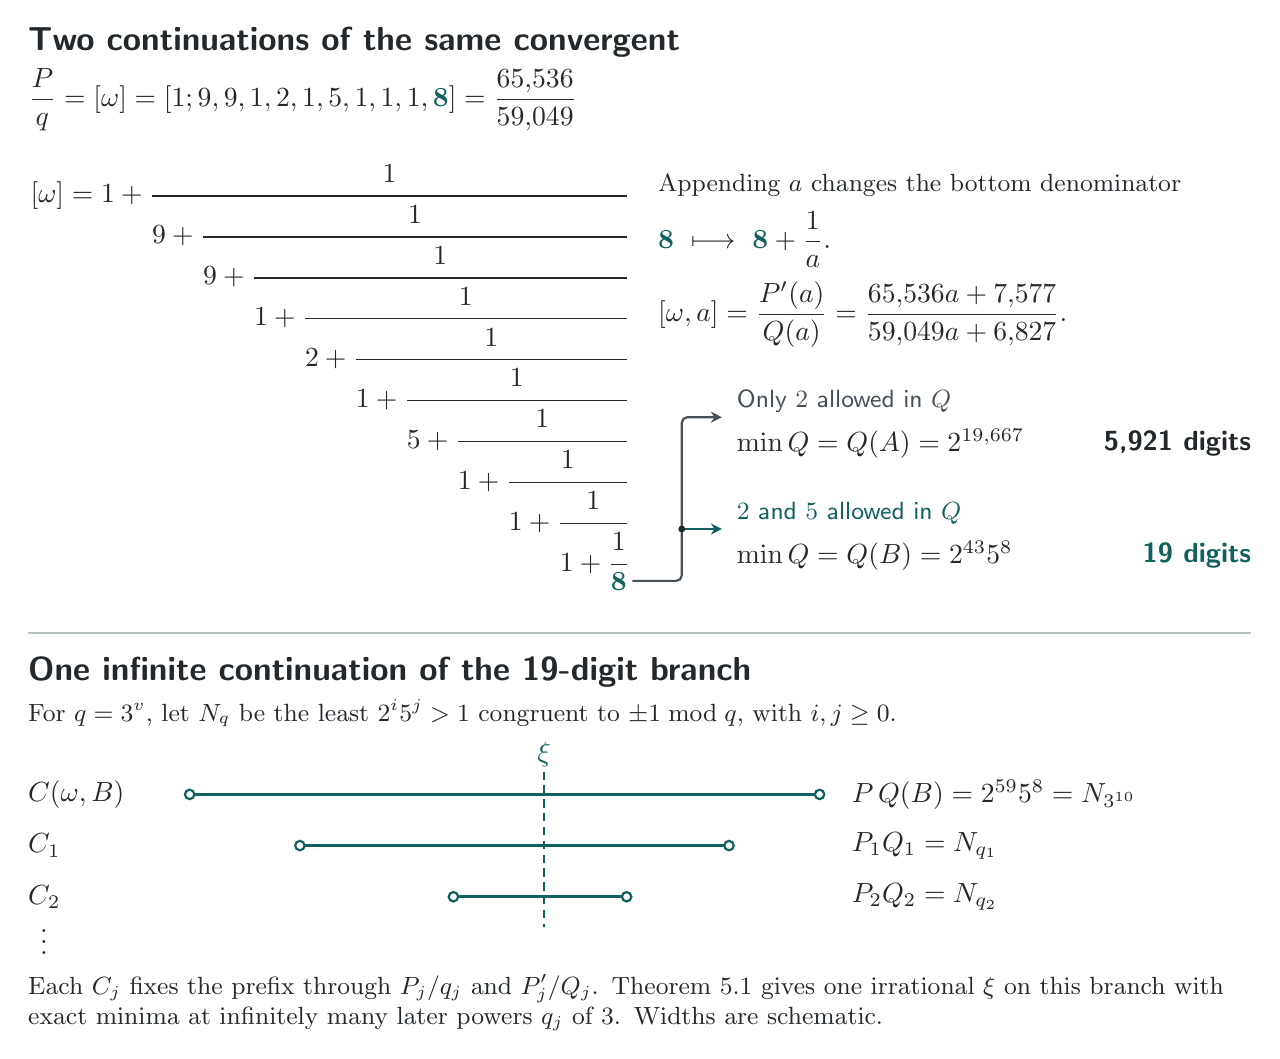
\begin{tikzpicture}[
    x=1cm,y=1cm,text=ink,
    every node/.style={inner sep=0pt,outer sep=0pt},
    heading/.style={anchor=west,font=\sffamily\bfseries\large},
    line text/.style={anchor=west,font=\small},
    branch label/.style={anchor=west,font=\sffamily\small},
    branch/.style={line width=.8pt,line cap=round,-{Stealth[length=4pt,width=4pt]}},
    interval/.style={draw=teal,line width=1.1pt},
    endpoint/.style={draw=teal,fill=white,line width=.8pt}
]
\node[heading] at (0,12.20) {Two continuations of the same convergent};
\node[anchor=west] at (0,11.47)
    {$\displaystyle \frac{P}{q}=[\omega]=[1;9,9,1,2,1,5,1,1,1,\textcolor{teal}{\mathbf{8}}]
      =\frac{65{,}536}{59{,}049}$};

\node[anchor=north west] (expanded) at (0.03,10.72) {$\displaystyle
    [\omega]=1+\reciprocal{9+
      \reciprocal{9+
        \reciprocal{1+
          \reciprocal{2+
            \reciprocal{1+
              \reciprocal{5+
                \reciprocal{1+
                  \reciprocal{1+
                    \reciprocal{1+
                      \reciprocal{\textcolor{teal}{\mathbf{8}}}
                    }
                  }
                }
              }
            }
          }
        }
      }
    }$};

\node[line text] at (8.00,10.38) {Appending $a$ changes the bottom denominator};
\node[anchor=west] at (8.00,9.70)
    {$\displaystyle \textcolor{teal}{\mathbf{8}}\ \longmapsto\
      \textcolor{teal}{\mathbf{8}}+\frac{1}{a}.$};
\node[anchor=west] at (8.00,8.74)
    {$\displaystyle [\omega,a]=\frac{P'(a)}{Q(a)}
      =\frac{65{,}536a+7{,}577}{59{,}049a+6{,}827}.$};

\coordinate (terminal) at ([xshift=2pt,yshift=3.5pt]expanded.south east);
\coordinate (fork) at (8.30,6.02);
\draw[muted,line width=.8pt,rounded corners=2pt] (terminal) -| (fork);
\draw[branch,muted,rounded corners=2pt] (fork) |- (8.81,7.44);
\draw[branch,teal] (fork) -- (8.81,6.02);
\fill[ink] (fork) circle (1.25pt);

\node[branch label,muted] at (9.00,7.64) {Only $2$ allowed in $Q$};
\node[anchor=west] at (9.00,7.10) {$\min Q=Q(A)=2^{19{,}667}$};
\node[anchor=east,font=\sffamily\bfseries] at (15.53,7.10) {5,921 digits};

\node[branch label,teal] at (9.00,6.22) {$2$ and $5$ allowed in $Q$};
\node[anchor=west] at (9.00,5.68) {$\min Q=Q(B)=2^{43}5^8$};
\node[anchor=east,font=\sffamily\bfseries,text=teal] at (15.53,5.68) {19 digits};

\draw[draw=rulegray,line width=.4pt] (0,4.70) -- (15.53,4.70);
\node[heading] at (0,4.20) {One infinite continuation of the 19-digit branch};
\node[line text] at (0,3.68)
    {For $q=3^v$, let $N_q$ be the least $2^i5^j>1$ congruent to $\pm1\bmod q$, with $i,j\ge0$.};

\node[text=teal] at (6.55,3.15) {$\xi$};
\draw[teal,densely dashed,line width=.6pt] (6.55,2.94) -- (6.55,0.97);
\foreach \height/\leftend/\rightend in {2.65/2.05/10.05,2.00/3.45/8.90,1.35/5.40/7.60}{
    \draw[interval] (\leftend,\height) -- (\rightend,\height);
    \draw[endpoint] (\leftend,\height) circle (1.7pt);
    \draw[endpoint] (\rightend,\height) circle (1.7pt);
}
\node[anchor=west] at (0,2.65) {$C(\omega,B)$};
\node[anchor=west] at (0,2.00) {$C_1$};
\node[anchor=west] at (0,1.35) {$C_2$};
\node at (.20,.88) {$\vdots$};
\node[anchor=west] at (10.46,2.65) {$P\,Q(B)=2^{59}5^8=N_{3^{10}}$};
\node[anchor=west] at (10.46,2.00) {$P_1Q_1=N_{q_1}$};
\node[anchor=west] at (10.46,1.35) {$P_2Q_2=N_{q_2}$};

\node[line text,text width=15.53cm,anchor=north west,align=left] at (0,.36)
    {Each $C_j$ fixes the prefix through $P_j/q_j$ and $P'_j/Q_j$. Theorem~5.1 gives
     one irrational $\xi$ on this branch with exact minima at infinitely many later
     powers $q_j$ of $3$. Widths are schematic.};
\end{tikzpicture}
\end{document}
